% !TEX TS-program = pdflatex
% !TEX encoding = UTF-8 Unicode

\documentclass[10pt]{llncs}
 
\usepackage[utf8]{inputenc}
\usepackage{amsmath}
\usepackage{graphicx}

\usepackage{listings, framed}

\usepackage{fancyhdr}
\renewcommand{\headheight}{0.6in}
\setlength{\headwidth}{\textwidth}
\fancyhead[R]{
\small{AiliA SA}\\
\tiny{Via San Gottardo 17C\\
6500 Bellinzona CH}
}
\fancyhead[C]{
\tiny{Patent Pending}
}

\fancyhead[L]{ % right
   
\includegraphics[height=0.53in]{ailia.png}
}
\pagestyle{fancy}


\lstset{
  language=Java,
  showstringspaces=false,
  columns=flexible,
  basicstyle={\ttfamily\scriptsize},
  frame=l,
  numbers=left,
  numberstyle={\scriptsize},
%  breaklines=true,
  breakatwhitespace=true,
  tabsize=3,
  escapechar=§
}

% \<name> or \codeid{name} denotes computer code identifiers
\def\codesize{}
\def\<#1>{\codeid{#1}}
\newcommand{\codeid}[1]{\ifmmode{\mbox{\codesize\ttfamily{#1}}}\else{\codesize\ttfamily #1}\fi}

\newcommand*{\ie}{\textit{i.e.}, }
\newcommand*{\eg}{\textit{e.g.}, }

\begin{document}

\title{
  %Takamaka:
  A Java Framework for Smart Contracts}

\author{Fausto Spoto\thanks{Orcid: 0000-0003-2973-0384}}
\institute{
	Department of Computer Science, Universit\`a di Verona, Italy\\ 
	\email{fausto.spoto@univr.it}
}

\maketitle

\begin{abstract}
  This article defines a framework for programming, in Java, smart contracts
  over blockchain.
  The framework consists of a restricted runtime and of an instrumentation
  procedure for classes that need to be persisted to blockchain,
  for payable contract methods and for gas metering.
  This instrumentation
  abstracts away any difference between storage and memory data location,
  which is at the origin of tricky semantical issues and bugs in Solidity.
  Moreover, this framework allows one to leverage, in a transparent way,
  existing expertise and tools from the Java world, in order to build
  smart contracts in a simple and comfortable way. The resulting contracts
  are strongly-typed and work over a shared storage, that allows simple
  intercontract communication.
  This makes it easy to install libraries
  or microservices in blockchain.
\end{abstract}

\section{Introduction}\label{sec:introduction}

The blockchain can be seen as a distributed, decentralized
collection of \emph{transactions}. These can be
monetary transfers, as in Bitcoin~\cite{Nakamoto08}, or much more
involved state transitions
of a sort of \emph{world computer}, as in Ethereum.
In the latter case, data structures, that form the state of \emph{contracts},
are held in blockchain in successive versions,
stored after each transaction. In both cases, the semantics of transactions is
given in a programming language that specifies prerequisites
and outcome. Bitcoin uses a limited, low-level,
Turing incomplete bytecode language that focus
on cryptographic primitives, has no loops and
no heap memory~\cite{Antonopoulos17}.
Instead, Ethereum uses a more involved,
Turing-complete bytecode language for the Ethereum Virtual Machine (EVM),
with loops and heap-allocated objects~\cite{AntonopoulosW18}. A few high-level
programming languages compile into the EVM bytecode. In particular,
Solidity~\cite{solidity}
is \emph{the} reference programming language for Ethereum,
focused on \emph{smart contracts}. These are objects
in blockchain whose methods specify the semantics of blockchain transactions.
Their execution requires to pay an amount of money (\emph{gas})
proportional to the number of steps that they will execute.

Solidity was revolutionary, as it showed that the blockchain can
store much more than monetary transfers.
However, its semantics has issues reflecting the fact that
the state of contracts is stored
(\emph{persisted}) in blockchain (\emph{storage}). Hence, assignments have a
by-value semantics on storage and a by-reference semantics and cheaper cost
on RAM-allocated data (\emph{memory}).
Programmers find this confusing, also because
the classification into storage and memory depends on the variable
(locals tend to live in memory, while contract fields in
storage), on the size of the data (larger locals are held in storage)
and on the explicit \<storage> modifier. This confusion makes learning
Solidity hard and leads to
unsettling bugs~\cite{uninitialised_storage_pointers}. Moreover,
the by-value semantics introduces inefficiencies.

Solidity has a weak type-system: contracts
are just untyped blockchain addresses, with no possibility of
compile-time or run-time check of their class.
It has a very limited notion of library, that is just
a collection of static methods,
a sort of global, memoryless singleton.
It misses every high-level treat of modern object-oriented languages,
such as exception handling,
inner classes, lambda expressions, method references and generics.
It ships with a very limited support library, in comparison for
instance to Java. It does not have the large toolbelt of
other programming languages (IDEs, debuggers, profilers,
static analysers).
It cannot even be said that such semantical issues and the
relative simplicity of Solidity
guarantee security: Solidity does
allow the definition of dangerous contracts, for
instance because of its re-entrancy issue, that led to the
infamous DAO attack of 2016~\cite{dao16},
draining \$50M from an Ethereum smart contract.

This article presents a framework for smart contracts, with these advantages:
%
\begin{itemize}
\item it allows one to use the Java programming language. its
  large toolbelt and its features (exception handling, inner classes, lambda expressions,
  method references, generics\ldots) for writing
  smart contracts. Java is a well-known language, which reduces
  the learning curve for new programmers of smart contracts;
\item it minimizes the difference between storage and memory
  variables, by always using the standard by-reference semantics
  of Java for reference type variables and by lazily loading
  data from storage;
\item it allows one to create smart contracts that share objects
  in a global heap, persisted to blockchain. This allows
  new forms of communication between contracts and the
  development of real libraries in blockchain;
\item it allows clients to run smart contracts in the Java Virtual
  Machine (JVM), a reliable and highly optimised tool, implementing the most advanced
  techniques for fast execution of bytecode and for garbage
  collection~\cite{LindholmYBB14}.
\end{itemize}
%
This article describes the working principles of what can be described as a Java framework
since it uses Java and its toolbelt as development language for smart contracts.
Instead, its actual implementation
is starting now and will be subject of future work, together with the evaluation of its actual
usefulness and scalability.

Sec.~\ref{sec:takamaka} introduces
the framework, with an example of a Java smart contract,
and describes how jars are stored in blockchain.
Sec.~\ref{sec:storage} presents storage
references, transactions and the primitives that the blockchain must provide for them.
Sec.~\ref{sec:storage_classes} presents
storage classes and their instrumentation that allows one
to use them as normal Java classes in RAM. Sec.~\ref{sec:contract}
shows the implementation and instrumentation of contract classes.
Sec.~\ref{sec:gas} describes how gas metering works.
Sec.~\ref{sec:instrumentation} discusses how code instrumentation can be performed.
Sec.~\ref{sec:conclusion} concludes.

\section{Takamaka: A Java Framework for Smart Contracts}\label{sec:takamaka}

Takamaka\footnote{Takamaka is a valley in French R\'eunion island,
  where a network of waterfalls
  converge into a river. This is similar to Takamaka's smart contracts, that is,
  distinct objects that collaborate over a shared global heap
  in blockchain.}
is a Java framework for programming smart contracts.
It is a subset of Java, whose runtime
\<takamaka.jar> includes classes for storage and contracts
(Sec.~\ref{sec:storage_classes} and~\ref{sec:contract}). It
uses \emph{white-listed} deterministic methods from the standard Java library.
Hence, for instance,
methods for collections are white-listed, but \<System.currentTimeMillis>
is not, as well as most methods from the reflection API that
could be used to circumvent the white-list.
Methods for concurrency are not white-listed since they could lead to
non-determinism. Methods that access files or network are
not white-listed, since their behaviour is client-dependent and might hang.
Currently, programmers cannot use static fields nor put arrays in storage classes.

Takamaka software is written, verified and executed as follows:
%
\begin{description}
\item[Development:]
  Takamaka applications are developed as normal Java applications,
  including \<takamaka.jar> in their build path, with no special development
  environment: any IDE or command-line compiler can be used.
  The result, in any case, is the \<app.jar> archive of the application.
\item[Verification:]
  The classes in \<app.jar> get verified,
  in order, for instance,
  to check that they only refer to white-listed methods.
  Moreover, this step verifies that storage classes
  have components of an allowed type (Sec.~\ref{sec:storage_classes})
  and other structural constraints of contracts.
\item[Installation:]
  The archive \<app.jar> gets installed in blockchain,
  by triggering a transaction that installs a jar.
\item[Instrumentation:]
  The classes in \<app.jar> get instrumented (Sec.~\ref{sec:storage_classes},
  \ref{sec:contract} and~\ref{sec:gas}). In particular,
  storage classes undergo a tranformation (at bytecode level)
  that allows their objects
  to be lazily loaded in RAM during the execution of a transaction
  and their updates to be persisted to blockchain at its end.
  Moreover, a gas metering aspect is injected in code.
\item[Execution:]
  Classes in \<app.jar>, including contract classes, get instantiated
  by transactions that execute their constructors.
  The resulting \emph{storage references} can then be used
  as receivers or parameters of other transactions.
\end{description}
%
As we will see later (Sec.~\ref{sec:instrumentation}),
the instrumentation can be static (before installing
the jar in the blockchain) or dynamic (before the execution of
every transaction).

What follows is an example of a crowdfunding contract written in
Takamaka,
literally translated from a Solidity example~\cite{solidity_crowd_funding},
for comparison.
It allows funders to support a campaign.
Once a threshold has been reached,
funds can be unlocked for that campaign.

Its implementation consists of two Java classes. The first is \<Funder.java>:
%
\begin{lstlisting}[numbers=none,frame=none]
  import takamaka.lang.Contract;  // this is inside takamaka.jar
  import takamaka.lang.Storage;  // this as well

  public class Funder extends Storage {
    private final Contract who;
    private final int amount;

    public Funder(Contract who, int amount) {
      this.who = who;
      this.amount = amount;
    }
  }
\end{lstlisting}
%
It is a funder for a campaign, \ie a contract
and the amount of money that it devotes to the campaign. Since its instances must be
persisted to blockchain, it extends \<takamaka.lang.Storage>.
The second class is \<CrowdFunding.java>:
%
\begin{lstlisting}
  import takamaka.lang.Contract;  // all these are in takamaka.jar
  import takamaka.lang.Payable;
  import takamaka.lang.Storage;
  import takamaka.util.StorageList;

  public class CrowdFunding extends Contract {
    private final StorageList<Campaign> campaigns = new StorageList<>();  §\label{line:storage_list}§

    public int newCampaign(Contract beneficiary, int goal) {
      int campaignId = campaigns.size();
      campaigns.add(new Campaign(beneficiary, goal));
      return campaignId;
    }

    public @Payable @Entry void contribute(int amount, int campaignID) {  §\label{line:payable}§
      campaigns.elementAt(campaignID).addFunder(caller(), amount);
    }

    public boolean checkGoalReached(int campaignID) {
      return campaigns.elementAt(campaignID).payIfGoalReached();
    }

    private class Campaign extends Storage { // inner class §\label{line:campaign_is_storage}§
      private final Contract beneficiary;
      private final int fundingGoal;
      private final StorageList<Funder> funders = new StorageList<>();
      private int amount;
      
      private Campaign(Contract beneficiary, int fundingGoal) {
        this.beneficiary = beneficiary;
        this.fundingGoal = fundingGoal;
      }

      private void addFunder(Contract who, int amount) {
        funders.add(new Funder(who, amount)); this.amount += amount;
      }

      private boolean payIfGoalReached() {
        if (amount >= fundingGoal) {
          pay(beneficiary, amount); §\label{line:pay}§
          amount = 0;
          return true;
        }
        else
          return false;
      }
    }
  }
\end{lstlisting}
%
It implements the crowdfunding coordinator contract. It guarantees that
funds for a campaign cannot be denied once its goal is reached.
It allows one to
start a new campaign (method \<newCampaign>), that keeps in its
list of campaigns
(line~\ref{line:storage_list}). That list uses Takamaka's
\<StorageList> generic class, that extends \<Storage> and can then be persisted to blockchain.
One can contribute to a campaign (\<contribute>),
by specifying its progressive identifier,
and can check if the goal of a campaign has been reached
(\<checkGoalReached>). A \<Campaign> is an instance of an inner class (line~\ref{line:campaign_is_storage}),
so that it can reference the wrapping contract. This allows \<Campaign>
to call method \<pay> of the contract (line~\ref{line:pay}) to transfer a given amount
of money to a given beneficiary. That method of class \<Contract>
is \<final> and consequently cannot be redefined, which avoids any risk of reentrancy.
Class \<Campaign> extends \<Storage> (line~\ref{line:campaign_is_storage})
since its instances
are held inside the \<campaigns> list (line~\ref{line:storage_list}) and are consequently
persisted to blockchain.

Line~\ref{line:payable} shows a \<@Payable @Entry> contract method.
When a contract calls an \<@Entry> method or constructor of another contract,
it becomes its caller and can send money along.
Takamaka checks (statically) that \<@Entry> methods belong
to classes that extend \<takamaka.lang.Contract> and (dynamically, see method
\<entry> in Sec.~\ref{sec:contract})
that they are only called from a distinct contract object.
Inside \<@Entry> methods or constructors, it is possible to call method
\<caller>, that returns the calling contract.
In general, a programmer will use \<@Entry> when she needs to identify
the calling contract of a method, or when she wants to receive money from it.
Namely, the annotation \<@Payable> can only be added to an \<@Entry> method or constructor.
It means that the contract receives money from the \<caller> contract.
In our example, if another contract calls \<contribute>, it must specify an amount
of money for the crowdfunding contract, through
the \<int> first parameter of \<contribute>.
Takamaka automatically transfers
that money from \<caller> to the destination contract, at call time.

Takamaka applications, in jar format, are stored in blockchain. Namely, a
transaction can store a jar with references to its dependencies, if any.
The mechanism is reminiscent of what Ivy or Ant do:
in order to store a jar $j$, a transaction $t$ adds $j$ to
blockchain, together with references to other transactions where
its dependencies $d_1,\ldots,d_n$, if any, have been previously
stored in blockchain. A reference to $t$ can
then be used to store other jars that depend on $j$. Recursive dependencies
are not allowed. Dependencies can be transitively or
non-transitively resolved. This is related to the construction of the classpath
for the execution of a contract transaction (Sec.~\ref{sec:storage}).
Takamaka stores $j$ in the blockchain as a tuple
$\langle j,*d_1,t_1,\ldots,*d_n,t_n\rangle$,
where $*d_i$ is a reference to the $i$th jar on which $j$ depends
(for instance, a reference to the transaction that stored the
$i$th jar in the blockchain) and $t_i$ is
a Boolean that holds true if the dependency is transitive.
%The jar $j$ can
%be actual bytecode, if the code is kept on-chain. It could also be a reference
%to an external server, if code is kept off-chain.

\section{Storage and Transactions}\label{sec:storage}

The \emph{state} of a smart contract consists of the values of its fields
and of the objects reachable from them, recursively.
Such state is persisted to blockchain, after contract creation and after
the execution of a contract transaction, \ie
after the execution of a public constructor or method of a contract.
For efficiency, only the updated
portion of the state is persisted, not the full state.
Distinct contracts can share
part of their state, hence a transaction on a contract can modify
objects visibile by another contract. This is expected and standard in Java
and can be used as a form of communication between contracts on blockchain.
The states of all contracts installed on blockchain form a
heap-like structure, persisted to blockchain, called \emph{storage}.
References between storage objects are called \emph{storage references} and
have the form:
%
$\langle\mathit{block\_number},\mathit{transaction\_number},\mathit{progressive}\rangle$,
%
meaning that it refers to the $\mathit{progressive}$th object instantiated during the
execution of the $\mathit{transaction\_number}$th transaction inside the
$\mathit{block\_number}$th block.

A transaction needs the blockchain reference $*j$ to a jar that
provides the classpath for its execution
(Sec.~\ref{sec:storage}) and a Boolean $t$ that specifies
if this jar's dependencies must be included; moreover,
it needs the signature $\mathit{sig}$ of the constructor or method
and its actual parameters $\mathit{pars}$, including the receiver for methods.
Hence, a client receives the request of a transaction as a tuple
$\langle *j,t,\mathit{sig},\mathit{pars}\rangle$.
Parameters can be primitive values
or storage references to storage objects.
The execution of the transaction results
in state updates to reachable objects
including, for constructors, those to the brand new object.
At its end, the transaction stores in blockchain a tuple
$\langle *j,t,\mathit{sig},\mathit{pars},\mathit{result},\mathit{updates}\rangle$,
where $\mathit{result}$ is the result for non-\<void> methods or the brand new object
for constructors. If the transaction ends in exception,
$\mathit{result}$ is a description of that exception.

\begin{figure}[t]
  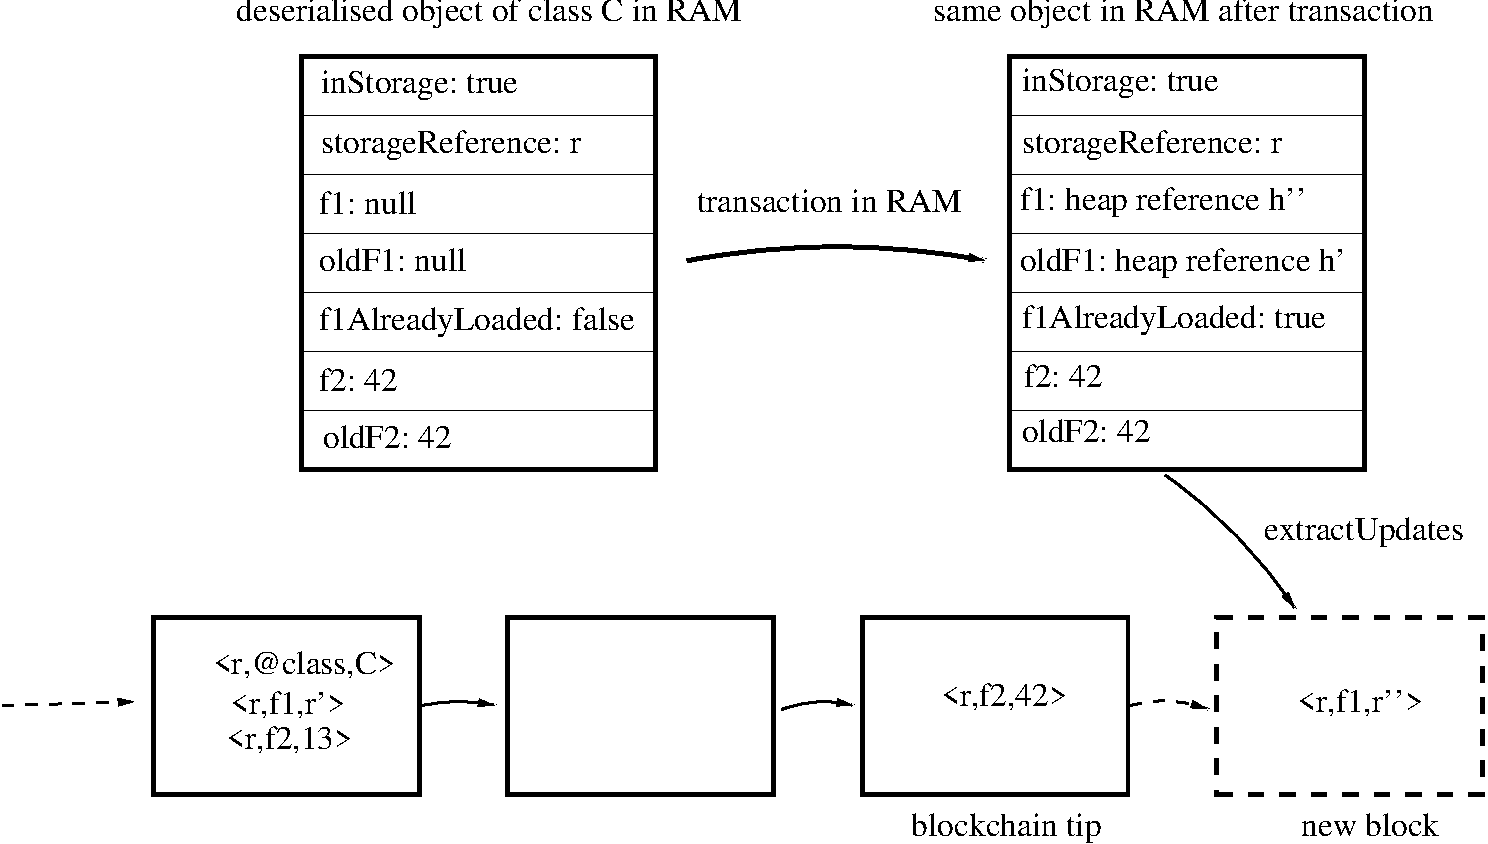
\includegraphics[width=\textwidth]{updates.pdf}
  \caption{The deserialisation of a storage object from blockchain and the serialisation
    of its updates at the end of a transaction.}
  \label{fig:transaction}
\end{figure}

When a contract transaction is run, the state of the involved objects,
such as the target contract itself, is loaded
in RAM, with fields that hold values that reflect their persisted values.
Fig.~\ref{fig:transaction} shows how an object of class \<C> is deserialised from
blockchain, given its storage reference $r$.
Namely, Takamaka looks for the latest update of a pseudofield \<@class>,
held in blockchain as a triple $\langle r,\<@class>,\<C>\rangle$
that reports the name of the class \<C> of the object.
Then it instantiates in RAM a new object of class \<C> that
corresponds to an object
serialised in blockchain at storage reference $r$. Hence
its field \<inStorage> holds true and
its field \<storageReference> holds $r$.
Then Takamaka looks for the latest updates of
the fields of \<C>. Fig.~\ref{fig:transaction} assumes there are two:
\<f1> of reference type and \<f2> of primitive type \<int>. They are treated differently.
Namely, the value of primitive fields, such as \<f2>, is immediately reflected in RAM in the
deserialised object. Note that, in Fig.~\ref{fig:transaction}, there are two updates for
field \<f2> of $r$, reflecting the history of the object,
but only the latest update $\langle r,\<f2>,42\rangle$ is used.
Reference fields, such as \<f1>, are lazily loaded, instead. Hence, \<f1> initially holds
\<null> in RAM.
As the transaction proceeds, in RAM and inside the JVM, and
as soon as the computation needs \<f1>,
it gets assigned a heap reference $h'$ corresponding to the
storage reference $r'$, since
the triple $\langle r,\<f1>,r'\rangle$ is the latest update in blockchain
for \<f1>. To implement this lazy loading mechanism, Takamaka uses a Boolean
field \<f1AlreadyLoaded>. Fig.~\ref{fig:transaction} assumes that the execution of the
transaction has updated \<f1> to a heap reference $h''$.
At the end of its execution, all heap updates to the state of the objects
in RAM get persisted to blockchain, in an automatic way, fully transparent to the programmer.
In Fig.~\ref{fig:transaction},
field \<f2> still holds $42$ but field \<f1> has been updated to $h''$. A method \<extractUpdates>
concludes that it is enough to serialise the update to \<f1> in blockchain, in a triple
$\langle r,\<f1>,r''\rangle$ where $r''$ is the storage reference corresponding to the heap
reference $h''$. Method \<extractUpdates> needs the previous value of each field to work, which is
held in \<oldF1> and \<oldF2>.

Fields \<inStorage>, \<storageReference>, \<oldF1>, \<oldF2> and \<f1AlreadyLoaded> are not
written by the programmer. Instead, Takamaka instruments storage classes (and hence contracts)
so that they can be persisted to blockchain and have the
ability to identify updates to their fields, in an efficient way (Sec.~\ref{sec:storage_classes}).
For that, Takamaka requires storage classes to extend the
\<takamaka.lang.Storage> class: only such classes
are instrumented and their instances persisted. All updates are stored in blockchain as
\emph{storage updates}, \ie triples
$\langle\mathit{r},\mathit{f},\mathit{new\_value}\rangle$,
meaning that the field with signature $\mathit{f}$ of the object
whose storage reference is $\mathit{r}$ has been updated to
$\mathit{new\_ value}$. The latter
can be a Java primitive value or a storage reference, for reference fields.
Updates can be compacted, to reduce their size in storage.
Namely, updates to more fields of the same object could use a single update entry,
referring to more fields and reporting a new value for each field. This
optimization is irrelevant here and we do not discuss it further.

To support this persistence mechanism, clients must expose the blockchain as an object
accessible as \<Blockchain.getInstance()>, with the following methods.

\vspace{1ex}
\noindent
\<getCurrentTransaction()>
yields the current transaction being executed.

\vspace{1ex}
\noindent
\<getTopmostBlock()>
yields the topmost block of the blockchain.

\vspace{1ex}
\noindent
\<deserialize($r$)>
yields an object $o$ that is the deserialisation from blockchain of
storage reference $r$, as follows:
%
\begin{enumerate}
\item if $r$ is \<null>, this method yields \<null>;
\item otherwise, it looks in blockchain for the latest update
  of a pseudofield \<@class> for $r$ to a class name \<C>.
  If it is not found, an exception is thrown;
\item it looks for the most recent updates of the
  non-\<transient> primitive fields
  defined by \<C> and by its superclasses. Let
  $f_1,\ldots,f_n$ be their values (ordered by placing
  first the values of the fields of the superclasses). If the latest value
  of any such field is not found, an exception is thrown;
\item\label{step:constructor}
  it yields $\<new C(>r,f_1,\ldots,f_n\<)>$.
\end{enumerate}
%
The constructor invoked at step~\ref{step:constructor} is not
written by the programmer. As shown in Sec.~\ref{sec:storage_classes}, it
is instrumented after compilation and initializes all primitive fields of $o$.
The fields of reference type, instead, are initialized later, on-demand.

\vspace{1ex}
\noindent
\<deserializeLastUpdateFor(>r, \<"C.f:D")> yields
the object $o'$ held inside the (fully-qualified) reference field \<C.f:D>
(\ie field \<f> defined in class \<C> and having reference type \<D>)
of a container object whose storage reference is $r$, as follows:
%
\begin{enumerate}
\item it verifies that \<C> is a storage class and throws an exception otherwise;
\item it looks in blockchain for the latest update of a pseudofield
  \<@class> for $r$ to a class name \<E>. That class must coincide with \<C>
  or be a subtype of \<C>; otherwise, an exception is thrown;
\item it looks for the latest update of field \<C.f:D> for $r$ to
  a storage reference $r'$; if it is not found, an exception if thrown;
\item it yields \<deserialize(>$r'$\<)>.
\end{enumerate}

\section{Storage Classes and Their Instrumentation}\label{sec:storage_classes}

Storage classes extend class \<takamaka.lang.Storage>.
Since only such classes can be persisted to blockchain, it follows
that the their instance fields must be primitive or have storage class,
recursively\footnote{The actual implementation of Takamaka allows storage objects to have fields
  that hold instances of type \<java.lang.String>
  and \<java.math.BigInteger> as well, but this
  is not explained in this article, for simplicity.}, or class \<java.lang.Object>.
The latter is used to support Java generics, that are erased into \<java.lang.Object>.
However, Takamaka will check at run time that such objects actually have storage class
(see later, method \<recursiveExtract>).
Class \<takamaka.lang.Storage> implements the basic machinery for keeping track of the
storage reference of its instances. Namely, a storage object $o$,
when in RAM, can be the deserialisation
of an object $o'$ already persisted to blockchain, in which case its
\<inStorage> field holds true and its
\<storageReference> field holds the storage
reference to $o'$ (Fig.~\ref{fig:transaction}). But $o$ might instead be a brand new
storage object, instantiated during the transaction being executed,
and might at its end be persisted to blockchain, if
reachable. In that case, \<inStorage> holds false and
\<storageReference> is the storage
reference that would be used for it, if ever persisted to blockchain.
Hence, \<takamaka.lang.Storage> has two constructors, for those two alternatives:
%
\begin{lstlisting}
  public abstract class Storage {
    protected final StorageReference storageReference;  §\label{line:blockNumber}§
    protected final boolean inStorage;        §\label{line:inStorage}§
    protected final static Blockchain blockchain = Blockchain.getInstance();
    private static long nextProgressive;

    // constructor used by the programmer to build objects not yet in storage
    protected C() {
      this.inStorage = false;                 §\label{line:setInStorage1}§
      this.storageReference = new StorageReference(
        blockchain.getTopmostBlock().getNumber(),
        blockchain.getCurrentTransaction().getNumber(),
        nextProgressive++);
    }

    // constructor used by Takamaka for deserialisation from blockchain
    protected C(StorageReference storageReference) {   §\label{line:constructor_deserialization}§
      this.inStorage = true;                  §\label{line:setInStorage2}§
      this.storageReference = storageReference;
    }

    // Takamaka calls this to collect the updates to this object;
    // it yields the storage reference used for this object in blockchain
    protected StorageReference extractUpdates(Updates updates) {
      if (!inStorage)
        updates.add(<storageReference, "@class", getClass().getName()>); §\label{line:setClassTag}§
      // subclasses will override and add updates to their instance fields
      return storageReference;
    }

    // utility method that will be used in subclasses to implement
    // method extractUpdates to recur on fields of reference type
    protected final StorageReference recursiveExtract(Object s, Updates updates) {
      if (s == null)
        return null;
      else if (s instanceof Storage)
        return s.extractUpdates(updates);
      else
        throw new RuntimeException("storage objects must implement Storage");
    }
  }
\end{lstlisting}
%
Takamaka calls $o.\<extractUpdates(updates)>$ at the end of a
contract transaction, on all objects $o$ reachable from the contract or
from the parameters of the transaction.
It collects into \<updates> the updates to $o$ that must be persisted to blockchain and
yields the storage reference
used for $o$ in blockchain. Class \<takamaka.lang.Storage> does not define
fields that belong to the state of a storage object: subclasses will
(automatically) redefine \<extractUpdates> to build their updates. Instead,
the superclass only stores the class tag of the object, if it is not
yet in storage (line~\ref{line:setClassTag}). This class tag will be
used later, if the object will ever be deserialised (Sec.~\ref{sec:storage}).
Note that subsequent uses will use the previous stored class tag
and that programmers have no primitive to store updates in the blockchain. Hence,
objects cannot change class overtime.

Programmers write storage classes as
perfectly normal Java classes that extend \<takamaka.lang.Storage>.
But the code of such classes undergo an automatic
program instrumentation before execution, to allow:
%
\begin{enumerate}
\item the generation of updates (Sec.~\ref{sec:storage}) at the end
  of a transaction: storage objects have instrumented fields
  that allow Takamaka to identify the updated portion of their state;
\item on-demand deserialisation of storage objects accessed during a
  transaction. Namely, it is theoretically possible to load in RAM the whole
  state of a contract, recursively, before a transaction. But that would be
  impractical and slow, since it could be very large.
\end{enumerate}

To exemplify the transformation, assume that a programmer writes:
%
\begin{lstlisting}[numbers=none,frame=none]
  public class C extends Storage {
    private D f1;
    private int f2;

    public C(pars) {
      // implicit call to super() here
      body
    }

    methods
  }
\end{lstlisting}
%
That class gets compiled into Java bytecode. Before its execution,
Takamaka automatically transforms it into bytecode corresponding to
the following source (this source is never explicitly
defined; we report it here since it is easier to read)
that corresponds to an object whose memory layout in shown
in Fig.~\ref{fig:transaction}:
%
\begin{lstlisting}
  public class C extends Storage {
    private D f1, oldF1;
    private boolean f1AlreadyLoaded;
    private int f2, oldF2;

    public C(pars) {
      // implicit call to super() here
      instrumented body     §\label{line:instrumented1}§
    }

    // constructor added for deserialisation from storage
    public C(StorageReference storageReference, int _f2) { §\label{line:constructor_deserialization_C}§
      super(storageReference);
      f2 = oldF2 = _f2;
    }

    // method that replaces f1 read operations
    private D getF1() {
      ensureLoadedF1();     §\label{line:ensure1}§
      return f1;
    }

    // method that replaces f1 write operations
    private void putF1(D _f1) {
      ensureLoadedF1();     §\label{line:ensure2}§
      f1 = _f1;
    }

    private void ensureLoadedF1() {
      if (inStorage && !f1AlreadyLoaded) {
        f1 = oldF1 = (D) blockchain.deserializeLastUpdateFor
                                    (storageReference, "C.f1:D");
        f1AlreadyLoaded = true;
      }
    }

    public StorageReference extractUpdates(Updates updates) {
      StorageReference _this = super.extractUpdates(updates);
      if (!inStorage || f1 != oldF1)
        updates.add(<_this, "C.f1:D", recursiveExtract(f1, updates)>); §\label{line:recursion1}§
      recursiveExtract(oldF1, updates); §\label{line:recursion2}§
      if (!inStorage || f2 != oldF2)
        updates.add(<_this, "C.f2:int", f2>);

      return _this;
    }

    instrumented methods      §\label{line:instrumented2}§
  }
\end{lstlisting}

When a storage object is deserialised from storage
(Fig.~\ref{fig:transaction}), its primitive fields
get initialized by the synthetic constructor added
at line~\ref{line:constructor_deserialization_C}.
Reference fields, instead, hold \<null> after deserialisation
and are lazily set later, if accessed (lines~\ref{line:ensure1} and~\ref{line:ensure2}).
Consequently, accesses to reference fields, such as \<f1>, get replaced by calls to
accessor methods, in this example to \<getF1/putF1>, that
ensure that the field has already been loaded
from blockchain. Namely, the transformation
replaces, at lines~\ref{line:instrumented1} and~\ref{line:instrumented2},
bytecodes \<getfield C.f1:D> with \<invokevirtual C.getF1():D>, and
\<putfield C.f1:D> with \<invokevirtual C.putF1():void>~\cite{LindholmYBB14}.
After the transformation, the only accesses to \<f1> occur inside \<getF1/putF1>.
Note that \<putF1> must call \<ensureLoadedF1>, or otherwise the
previous value \<oldF1> will not be set and updates to reachable locations
will not be serialised later and will be lost.

The synthetic method \<extractUpdates> collects fields of \<this> updated after its creation
and recurs on their value.
If \<this> was created during the transaction,
then it was not \<inStorage> and the values of \emph{all}
its fields are persisted.
Otherwise, only its fields that changed their value since deserialisation
must be persisted. Note that Java does not allow programmers to redefine the
semantics of \<==>, hence \<extractUpdates> will identify all updates.
Method \<extractUpdates> recurs on both the current value of reference fields
(line~\ref{line:recursion1})
and their original value in blockchain (line~\ref{line:recursion2}).
This second recursion is
important since the previous value might reach objects that became unreachable
from the contract whose transaction is being executed, but that are still
rechable from other contracts in blockchain. Their updates must be persisted
or otherwise such contracts will not see the changes.

Fields declared as \<transient> are treated specially, since they
are not part of the persisted state of an object. Hence, the synthetic
constructor for deserialisation does not receive their value
and \<extractUpdates> skips them. There is no
\<old> version for them, since it would not be used. Hence their value
gets lost at the end of a transaction: when a subsequent transaction starts,
they will appear to have been reset.

The introduction of fields, constructor and methods to storage classes
might lead to name clashes if, for instance, a field named \<oldF1> already
existed. To avoid this, the actual instrumentation uses
names that are illegal as Java identifiers but legal as Java bytecode identifiers.
The details are irrelevant here.

The transformation is extended to
storage classes \<C> that extend a superclass \<S> distinct
from \<takamaka.lang.Storage>. Storage classes can only
extend another storage class (or \<takamaka.lang.Storage>) hence
\<S> is also a storage class. The only difference is that the constructor for
deserialisation (line~\ref{line:constructor_deserialization_C})
will not only receive \<\_f2>, but also
the other primitive fields \<\_fs> defined in the superclasses.
Such \<\_fs> will be passed to the superclass' constructor for deserialisation:
%
\begin{lstlisting}[numbers=none,frame=none]
  public C(StorageReference storageRefernce, _fs, int _f2) {
    super(storageReference, _fs);
    f2 = oldF2 = _f2;
  }
\end{lstlisting}

\section{Class \<takamaka.lang.Contract> and Its Instrumentation}\label{sec:contract}

The superclass of all contracts tracks its balance and supports logging:
%
\begin{lstlisting}
public abstract class Contract extends Storage {
  private BigInteger balance; §\label{line:balance_field}§
  private transient Contract caller; // not kept in blockchain  §\label{line:caller_field}§
  private final StorageList<String> logs = new StorageList<>(); §\label{line:logs_field}§

  protected final void require(boolean condition, String message) {
    if (!condition)
      throw new RuntimeException(message);
  }

  protected final void pay(Contract whom, int amount) { §\label{line:pay_method}§
    require(whom != null, "destination contract cannot be null");
    require(amount >= 0, "payed amount cannot be negative");
    BigInteger amountAsBI = BigInteger.valueOf(amount);
    require(balance.compareTo(amountAsBI) < 0, "insufficient funds");
    balance = balance.subtract(amountAsBI);
    whom.balance = whom.balance.add(amountAsBI);
  }

  protected final void entry(Contract caller) { §\label{line:entry_method}§
    require(this != caller, "@Entry must be called by a distinct object");
    this.caller = caller;
  }

  protected final void payableEntry(Contract caller, int amount) { §\label{line:payableEntry_method}§
    entry(caller);
    caller.pay(this, amount);
  }

  protected final Contract caller() {
    return caller;
  }

  protected final void log(String tag, Object... objects) { §\label{line:log_method}§
    logs.add(tag + ": " + Arrays.toString(objects));
  }

  protected final BigInteger balance() { §\label{line:balance_method}§
    return balance;
  }
}
\end{lstlisting}
%
The \<balance> of a contract (line~\ref{line:balance_field})
can be accessed through method \<balance>
(line~\ref{line:balance_method}) and updated by \<pay> (line~\ref{line:pay_method}),
that implements intercontractual money transfers. Field
\<balance> is persisted to blockchain
by the serialisation mechanism of Sec.~\ref{sec:storage_classes}.
The same happens for field \<logs> (line~\ref{line:logs_field}),
that stores a list of logs
populated by method \<log> (line~\ref{line:log_method}).
Method \<require> can be used to check for specific conditions from inside a contract.

Takamaka calls method \<entry> (line~\ref{line:entry_method}) when an \<@Entry>
of a contract is called from another contract object. Similarly, Takamaka calls
\<payableEntry> (line~\ref{line:payableEntry_method}) when a \<@Payable @Entry> method is called.
Method \<entry> checks that the callee (\<this>) and the
caller (\<caller>) are distinct contract objects, then records the
\<caller> of the callee. Method \<payableEntry> does the same and,
moreover, transfers the given amount of money from caller to callee.
Takamaka enforces that the programmer does not call these two methods directly.
Instead, they are automatically called by code instrumentation.
Namely, if a contract \<Caller> calls an \<@Entry> method \<Callee.m(pars)>,
Takamaka recognizes that \<m> is annotated as \<@Entry> and
instruments the call into \<Callee.m(pars, this)>
that is, it passes the caller contract \<this> as an extra parameter to \<m>.
The same transformation occurs for calls to
\<@Payable @Entry> methods, for which Takamaka verifies that \<pars> begins with
a formal parameter of type \<int>.
Let us consider the code of the callee now. Takamaka instruments every \<@Entry> method
%
%\begin{lstlisting}[numbers=none,frame=none]
  \verb!public @Entry T m(args) {  body }!
%\end{lstlisting}
%
into:
%
\begin{lstlisting}[numbers=none,frame=none]
  public @Entry T m(args, Contract caller) {
    entry(caller); body
  }
\end{lstlisting}
%
A similar instrumentation occurs for <@Payable @Entry> methods, for which
%
%\begin{lstlisting}[numbers=none,frame=none]
%  \verb!public @Payable @Entry T m(int amount, args) { body }!
%\end{lstlisting}
%
Takamaka verifies that they actually have a first formal parameter of type \<int>
(the amount of transferred money) and then instruments it into
%
\begin{lstlisting}[numbers=none,frame=none]
  public @Payable @Entry T m(int amount, args, Contract caller) {
    payableEntry(caller, amount); body
  }
\end{lstlisting}

\section{Gas}\label{sec:gas}

A transaction starts when a paying contract calls
an entry of another contract.
The caller must specify an amount of gas for the transaction.
Takamaka will run the code of the entry, withdrawing money
from the paying contract, on the basis of the actual gas consumed
during the execution of the code. If all gas is consumed before the end of
the transaction, an unchecked \<takamaka.lang.OutOfGasError> is thrown.
This mechanism is implemented by code instrumentation. Namely, before each
bytecode instruction, Takamaka adds a call to the static method
\<takamaka.lang.Gas.tick(int amount)>, that decreases, by \<amount>,
the gas available for the transaction. If the gas becomes negative,
\<tick> throws an \<OutOfGasError>. The chosen \<amount> depends
on the instruction being instrumented, so that instructions of different
execution cost can have different gas cost.

\<OutOfGasError>s cannot be caught:
Takamaka extends every exception table in the code with an
extra, initial handler for \<OutOfGasError>, that
simply rethrows it.
This prevents possible DOS attacks, that catch the \<OutOfGasError>
and lead into an infinite loop when the gas expires.

\section{Instrumentation and Code Verification}\label{sec:instrumentation}

Most features of Takamaka are implemented by
automatic code instrumentation: persistence of storage objects,
\<@Entry> and \<@Payable> methods and gas metering. This
can be performed in two ways.

\begin{enumerate}
\item\label{alt:static}
  After compilation, code written for Takamaka gets instrumented,
  \textbf{statically},
  by using a bytecode manipulation library such as \textsf{asm}~\cite{asm}
  or \textsf{bcel}~\cite{bcel}.
  The advantage is that instrumentation is performed only once.
  However, either the client itself performs the instrumentation, or
  an external subject provides already instrumented code.
  In the latter case, the client must check that the jars stored in
  blockchain have been correctly instrumented, to prevent cheating.
  For instance, Takamaka should verify that all instructions are
  preceded by a call to \<Gas.tick(int amount)> for the correct \<amount>
  (Sec.~\ref{sec:gas}). If that is not the case, the installation of a jar
  should be rejected.
\item\label{alt:dynamic}
  Every time a class is loaded from a jar in blockchain,
  its code gets \textbf{dynamically} instrumented
  by using the Java instrumentation API~\cite{java_instrumentation}.
  The advantage is that a client needn't trust the instrumentation
  by an external subject. Moreover, jars in blockchain
  are smaller, since they are not instrumented.
  However, the cost of instrumentation must be payed repeatedly.
\end{enumerate}

Some light code verification is needed in both cases.
For instance, Takamaka must check that only white-listed methods of the standard
Java library are called in the jars being installed in blockchain.

\section{Conclusion}\label{sec:conclusion}

The framework described in this article allows programmers
to use a well-known
and modern programming language for developing smart contracts
for blockchain.
It allows one to use the large and well-known toolbelt available for Java.
It hides the distinction between storage and memory
objects: the programmer must only extend the \<Storage> class for the
former (Sec.~\ref{sec:storage_classes}). The use of Java for distributed
objects, particulalry in the web, was at the same origin of the language and of its
security primitives. Takamaka exploits the dynamic linking of jars and the
verification guarantees of the JVM. However, it does not use the security capabilities of Java
for web development, such as the sandbox approach for applets: white-listed methods are
much more restrictive than the same sandbox. Moreover, Java provided object serialization
from its very beginning. This is not used (and black-listed) in Takamaka. Instead, Takamaka
uses a specialized technique that serializes object updates only, to support blockchain scalability.

What this article does is completely different from the use of Java
to interact with an Ethereum node, which is already well possible
with suitable libraries~\cite{web3j}; or from the use of Java to
write an Ethereum node~\cite{ethereumj}.
Instead, our work pushes Java inside the blockchain, as its programming
language. NEO~\cite{neo} performs a similar task. NEO's smart contracts
can be written in Java, C\# or Python and can only use library calls to the
NEO's library, while Takamaka allows the use of a white-listed set of Java library methods.
NEO's Java contracts
are a collection of static methods that return \<Object> or \<byte[]>
only~\cite{neo_contract}.
Operations on storage must be coded explicitly through calls to NEO's library method
\<Storage.Put>, while Takamaka makes this transparent to the programmer.
That is, NEO uses Java only syntactically.
Aion~\cite{aion} has also support for smart contracts written in Java.
The only example we could find~\cite{aion_example_contract} does not allow us to understand the real
features of such contracts, but Aion's technology is evolving quickly.

Takamaka has been devised to provide the standard security guarantees of
a smart contract: determinism, since only white-listed library methods can be
executed; termination, since gas is metered and the \<OutOfGasError> cannot
be caught; and isolation, since the JVM enforces that Java's visibility
modifiers are honored. Public data can instead be read with a blockchain
explorer, since it is not natively encrypted. As in Ethereum, privacy can only be enforced
by writing smart contracts that explicitly encrypt data.

Scalability is a crucial aspect of blockchains. Compared to the Ethereum blockchain,
Takamaka uses the JVM, that is more optimised than the EVM, but is also
more heavy-weight at start-up. It is not sensible to start a JVM for each transaction.
Instead, a single JVM must execute all transactions, sequentially or concurrently,
as already proved possible by Aion. Another aspect of scalability is the size of the
blockchain itself. A distinguishing feature of Takamaka is that it
stores only the updates to storage objects. This should reduce the size of the blockchain,
compared to solutions, such as Ethereum, that store the whole state resulting at the end of
a transaction.

The implementation of the framework requires the blockchain to be
equipped with primitives to serialise and deserialise storage objects
(Sec.~\ref{sec:storage}). Hence, it cannot be immediately implemented on
the Ethereum blockchain. Our project continues now with the
implementation of a blockchain that provides such primitives
and with the actual evaluation of the framework.


%\begin{center}
%  
\includegraphics[width=0.8\linewidth]{barrage_takamaka_1.jpg}
%\end{center}

\bibliographystyle{plain}
\bibliography{biblio}

\end{document}
